\section{Evaluation}
\label{sec:eval}

In this section, we use simulations to characterize the performance of each of our three recovery algorithms in terms of message and time overhead. 
Our goal is to illustrate the relative performance of our recovery algorithms over different topology types (e.g., \er graphs, Internet-like graphs) and
different network conditions (e.g., fixed link costs, changing link costs).


%We build a custom simulator with a synchronous communication model: nodes send and receive messages at fixed epochs.  In each epoch, a node receives a
%message from all its neighbors and performs its local computation.  In
%the next epoch, the node sends a message (if needed).   All algorithms
We build a custom simulator with a synchronous communication model as described in Section \ref{sec:analysis}. All algorithms
are deterministic under this communication model.
The synchronous communication model, although simple, yields
interesting insights into the performance of each of the recovery
algorithms. Evaluation of our algorithms using a more general
asynchronous communication model is currently under
investigation. However, we believe an asynchronous implementation
will demonstrate similar trends.  

%Except in the case where multiple nodes are compromised, we simulate the following scenario:
We simulate the following scenario: 
{\footnote {\small In Section \ref{subsubsec:many} we consider the case of multiple compromised nodes.  In that experiment we modify our simulation scenario
to consider a set of compromised nodes, $\overline{V}$, instead of \bads.}}
\begin{enumerate}
	\item Before $t'$, $\forall v \in V$ \minvv and \dmatrixv are correctly computed.

	\item At time $t'$, \bad is compromised and advertises a \badvector (a vector with a cost of $1$ to \emph{every} node in the network) to its neighboring nodes.

	\item \badvector spreads for a specified number of hops (this varies by experiment).  Variable $k$ refers to the number of hops that \badvector has spread.

	\item At time $t$, some node $v \in V$ notifies all $v \in adj($\bads$)$ that \bad was compromised. 
	{\footnote { \small For \cpr this node also indicates the time, $t'$, \bad was compromised.}} 

\end{enumerate}
The message and time overhead are measured in step (4) above. The pre-computation common to all three recovery algorithms, described in Section \ref{subsec:preprocess},
is not counted towards message and time overhead. We describe our simulation scenario for multiple compromised nodes in Section \ref{subsubsec:many}.


\subsection{Fixed Link Weight Experiments}
\label{subsec:fixed}

In the next five experiments, we evaluate our recovery algorithms over different topology types in the case of fixed link costs.

\subsubsection{Experiment 1 - \er Graphs with Fixed Unit Link Weights}
\label{subsubsec:expt1}

We start with a simplified setting and consider 
Erd\"{o}s-R\'enyi graphs with parameters $n$ and $p$. 
$n$ is the number of graph nodes and $p$ is the probability that link $(i,j)$ exists where $i,j \in V$.
The link weight of each edge in the graph is set to $50$.
We iterate over different values of $k$. For each $k$, we 
generate an Erd\"{o}s-R\'enyi graph, $G = (V,E)$, with parameters $n$ and $p$. Then we select a \bad $\in V$ uniformly at random and simulate the scenario described above, 
using \bad as the compromised node. In total we sample $20$ unique nodes for each $G$.
We set $n=100$, $p=\{0.05,0.15,0.25, 0.50\}$, and let $k=\{1,2,
... 10\}$. Each data point is an average over $600$ runs ($20$ runs over 
$30$ topologies).  We then plot the $90 \%$ confidence interval.

For each of our recovery algorithms, Figure \ref{fig:msg} shows the
message overhead for different values of $k$. %The $90 \%$ confidence interval is shown.
We conclude that \cpr outperforms \purge and \second across all topologies. \cpr performs well because \badvector is removed using a single diffusing computation,  
while the other algorithms remove \badvector state through distance vector's iterative process.
\cprs's global state after rolling back is almost the same as the final recovered state.

\begin{figure*}[t]
\centering
\subfigure[{$p=0.05$, diameter=$6.14$}]{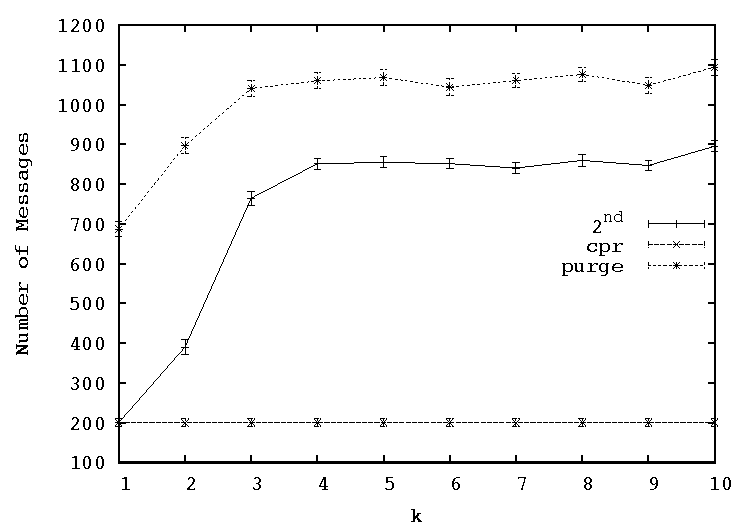
\includegraphics[width=0.32\textwidth]{figs/synch/msg5.pdf}}
\subfigure[{$p=0.15$, diameter=$3.01$}]{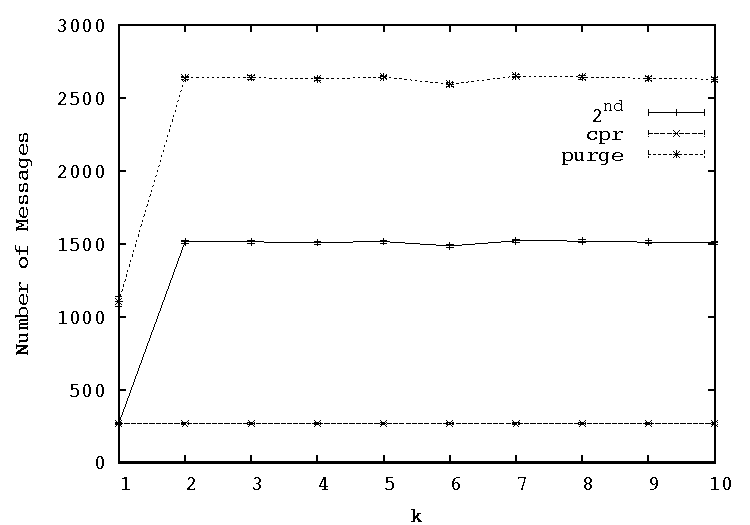
\includegraphics[width=0.32\textwidth]{figs/synch/msg15.pdf}}
\subfigure[{$p=0.25$, diameter=$2.99$}]{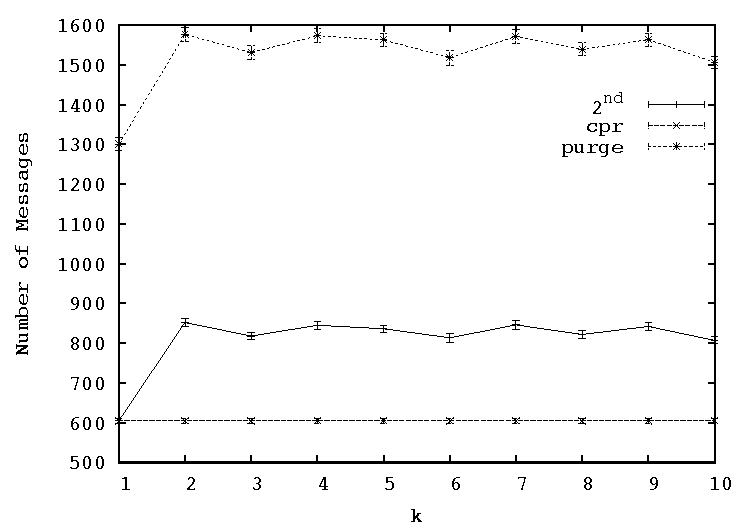
\includegraphics[width=0.32\textwidth]{figs/synch/msg25.pdf}}
\subfigure[{$p=0.50$, diameter=$2$}]{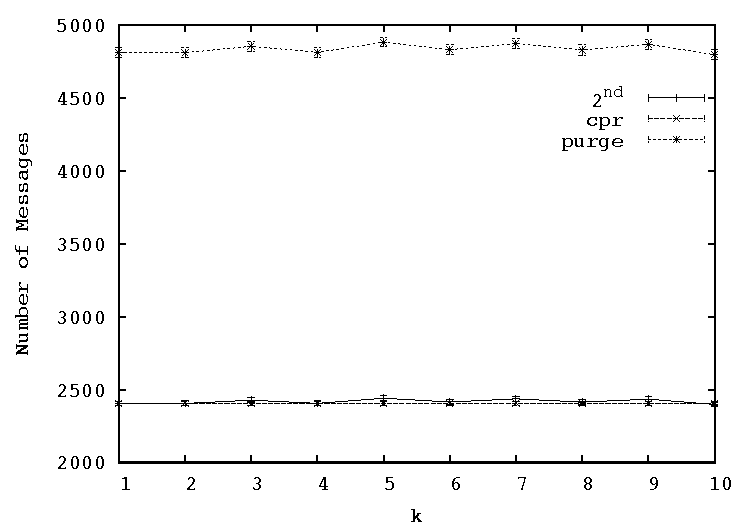
\includegraphics[width=0.32\textwidth]{figs/synch/msg50.pdf}}
%\subfigure[{Cumulative path cost decreases during the simulation}]{\includegraphics[width=0.49\textwidth]{figs/tsdecrease6.pdf}}
\caption{Experiment 1: message overhead for \er Graphs with Fixed Unit Link Weights generated over different $p$ values. Note the y-axis have different scales.}
\label{fig:msg}
\end{figure*}

\begin{figure*}[t]
\centering
\subfigure[{$p=0.05$, diameter=$6.14$}]{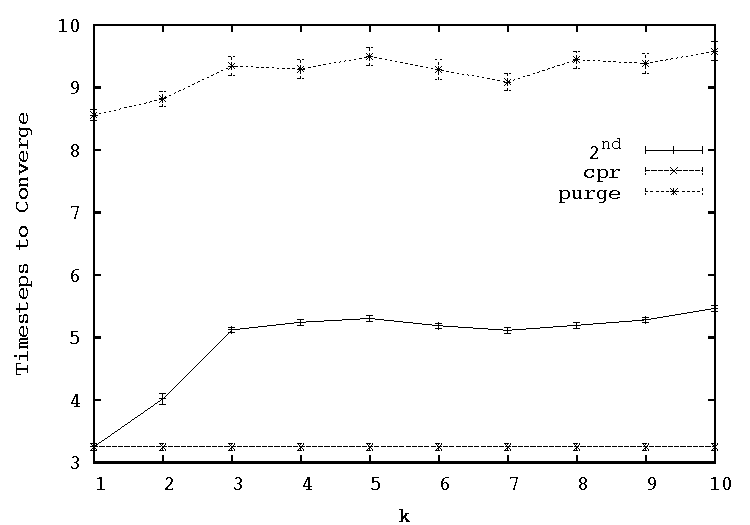
\includegraphics[width=0.32\textwidth]{figs/synch/epoch5.pdf}}
\subfigure[{$p=0.15$}, diameter=$3.01$]{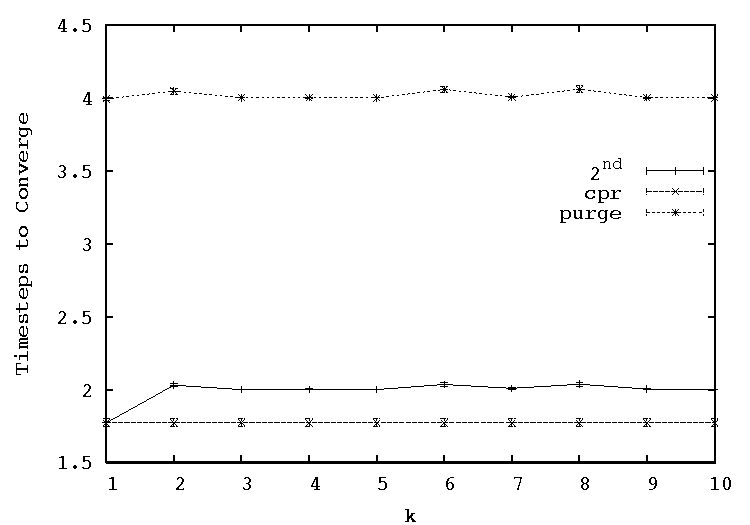
\includegraphics[width=0.32\textwidth]{figs/synch/epoch15.pdf}}
\subfigure[{$p=0.25$}, diameter=$2.99$]{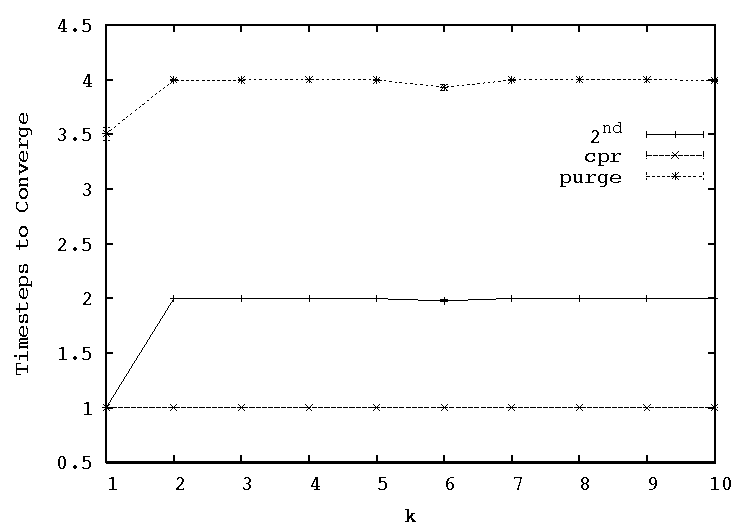
\includegraphics[width=0.32\textwidth]{figs/synch/epoch25.pdf}}
\subfigure[{$p=0.50$}, diameter=$2$]{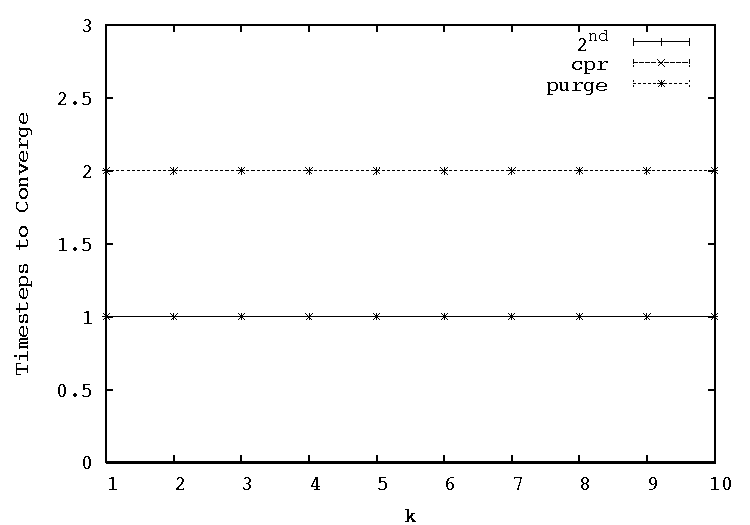
\includegraphics[width=0.32\textwidth]{figs/synch/epoch50.pdf}}
%\subfigure[{Cumulative path cost decreases during the simulation}]{\includegraphics[width=0.49\textwidth]{figs/tsdecrease6.pdf}}
\caption{Experiment 1: time overhead for \er Graphs with Fixed Unit Link Weights generated over different $p$ values.}
\label{fig:epoch}
\end{figure*} 


%In other words, \cpr performs well because its global state  (recall we define the global state of the routers as the union of their local states) is almost the same as the final recovered state.
%Specifically, if we let $S'$ represent the global state after rolling back and let $S$ be the final recovered state, the only difference between $S$ and $S'$, is that $S'$ 
%contains state that depends directly or transitively on \oldvector while $S$ does not. 
%\cpr performs exactly the same as \second at $k=1$ because \second at $k=1$ also must only remove \oldvector state and uses the same iterative process as \cprs. 
%For this reason, across all $k$ values, \cpr performs exactly the same as \second at $k=1$.  {\bf note:} {\it may need to elaborate more here.}

\second recovery can be understood as follows.  By Corollary \ref{cor:startbad} and \ref{cor:during} in Section \ref{subsec:trends}, distance values increase from their initial value until they 
reach their final (correct) value. Any intermediate, non-final, distance value uses \badvector or \oldvectors. Because \badvector and \oldvector no longer exist during recovery,
these intermediate values must correspond to routing loops.
%In this experiment, with \second distance estimates quickly count up to their final value.
Table \ref{tab:loop1} shows that there are few pairwise routing loops during \second recovery in the network scenarios generated in Experiment 1, 
indicating that \second distance values quickly count up to their final value.
{\footnote {\small We compute this metric as follows. After each simulation timestep, we count all pairwise routing loops over all source-destination pairs and then sum all of these values.}}
Although no pairwise routing loops exist during \purge recovery, \purge incurs overhead in performing network-wide state invalidation. Roughly, $50\%$ of \purges's messages come from these
diffusing computations. 
For these reasons, \purge has higher message overhead than \seconds.

Figure \ref{fig:epoch} shows the time overhead for the same $p$ values. The trends for time overhead match the trends we observe for message overhead. 
{\footnote {\small For the remaining experiments, we omit time overhead plots because time overhead follows the same trends as message overhead.}}


\begin{table}
\begin{center}
\begin{tabular}{l|l|l|l|l}
 & $k=1$&  $k=2$ & $k=3$ & $k=4-10$ \\
\hline
 $p=0.05$  & $0$ & $14$ & $87$ &  $92$ \\
 $p=0.15$  & $0$ & $7$&  $8$ & $9$ \\
 $p=0.25$  & $0$ & $0$ & $0$ &  $0$ \\
 $p=0.50$  & $0$ & $0$ & $0$ &  $0$ \\
 %$p=\{0.15,0.25,0.50\}$  & $0$ & $0$&  $0$ & $0$ \\
\end{tabular}
\end{center}
\caption{Average number pairwise routing loops for \second in Experiment 1.}
%$p=.50$ for Experiment 1 is omitted because no pairwise routing loops are found across all $k$ values.} 
\label{tab:loop1}
\end{table}

\begin{table}
\begin{center}
\begin{tabular}{l|l|l|l|l}
 & $k=1$&  $k=2$ & $k=3$ & $k=4-10$ \\
\hline
  $p=0.05$  & $554$ & $1303$ & $9239$ &  $12641$ \\
 $p=0.15$  & $319$ & $698$&  $5514$ & $7935$ \\
 $p=0.25$  & $280$ & $446$ & $3510$ &  $5440$ \\
 $p=0.50$  & $114$ & $234$ & $2063$ &  $2892$ \\
 %$p=\{0.15,0.25,0.50\}$  & $0$ & $0$&  $0$ & $0$ \\
\end{tabular}
\end{center}
\caption{Average number pairwise routing loops for \second in Experiment 2.}
%$p=.50$ for Experiment 1 is omitted because no pairwise routing loops are found across all $k$ values.} 
\label{tab:loop2}
\end{table}


\purge and \second message overhead increases with larger $k$. Larger $k$ imply that false state has propagated further in the network, 
implying more paths to repair, and therefore increased messaging.
For values of $k$ greater than a graph's diameter, the message overhead remains constant, as expected. 

%However, once $k$ is equal the graph diameter, $d$, the message overhead and number of epochs do not change for larger values of $k$ for a given topology. By definition, the graph diameter is
%the longest shortest path and so it follows that when $k > d$, each $v \in V'$ has a path less than $k$ hops to all destinations.  Therefore each $v$, does not use the $k$ hop path to \bads.
%For this reason, the message overhead (and number of epochs) do not change for $k>d$. {\bf todo verify if this is correct}

%Figure \ref{fig:compare} shows that for most values of $k$, if we do not count the epochs that occurred during \purges's purge phase 
%(e.g., only count \purges's discovery phase epochs), the resulting epoch omplexity is lower than \seconds's epoch complexity. When $k>2$, \second has higher epoch complexity 
%because the \infinity problem occurs with \second and not with \purges.  Table \ref{tab:loop1} shows that when $k>2$ there are pairwise routing loops during \second recovery, while

%The exception to this trend is when $k=1$ for all topologies and $k=2$ for $p=.05$: \purges's discovery phase epoch complexity is higher than \seconds's total epoch complexity. 
%In these cases, there are no or few pairwise routing loops for \seconds.  In this way, this is an ideal case for \second recovery. 
%Meanwhile, there are several cases in which distance values that previously used \oldvectors, which do not require messaging for \second but do for \purges.  
%Recall that \purge sets all distances that use \badvector or \oldvector to $\infty$ in its purge phase, so for \purge all distances using \oldvector must be recomputed. 
%With \seconds, many of these same distance values do not require re-computation: the actual path changes such as not to use \oldvector but the distance does not change because an 
%alternate path of the same distance is locally selected (since the distance does not change, no message is sent).


\subsubsection{Experiment 2 - \er Graphs with Fixed but Randomly Chosen Link Weights}
\label{subsec:expt2}


The experimental setup is identical to Experiment 1 with one exception: link weights are selected uniformly at random between $[1,n]$ (rather than using 
fixed link weight of $50$).

Figure \ref{fig:msg-rand} show the message overhead for different $k$ where $p=\{0.05,0.15,0.25,0.50 \}$. 
%We omit the figures for the other $p$ values because they follow the same trend as $p=.05$.
In striking contrast to Experiment 1, \purge outperforms \second for most values of $k$. 
\second performs poorly because the \infinity problem: Table \ref{tab:loop2} shows the large average number of pairwise routing loops in this experiment, 
an indicator of the occurrence of \infinity problem.
In the few cases (e.g., $k=1$ for $p=0.15$, $p=0.25$ and $p=0.50$) that \second performs better than \purges, \second has few routing loops.

No routing loops are found with \purges. \cpr performs well for the same reasons described in Section \ref{subsubsec:expt1}.  

\begin{figure*}[t]
\centering
\subfigure[{$p=0.05$, diameter=$6.14$}]{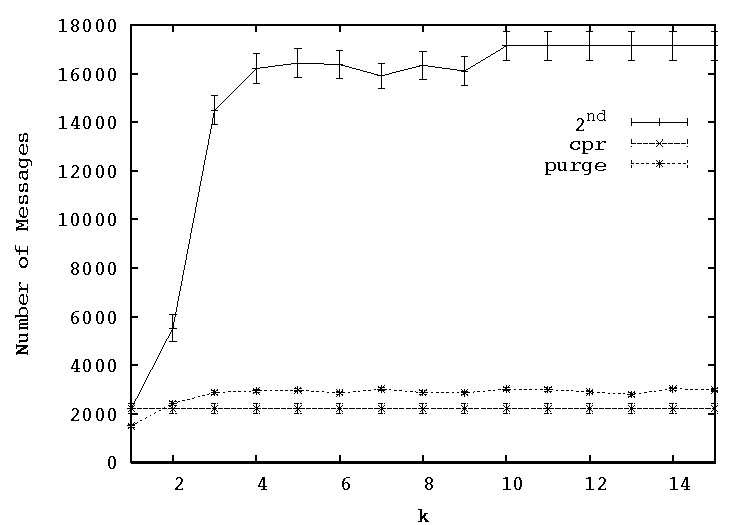
\includegraphics[width=0.32\textwidth]{figs/synch/msg-rand5.pdf}}
\subfigure[{$p=0.15$, diameter=$3.01$}]{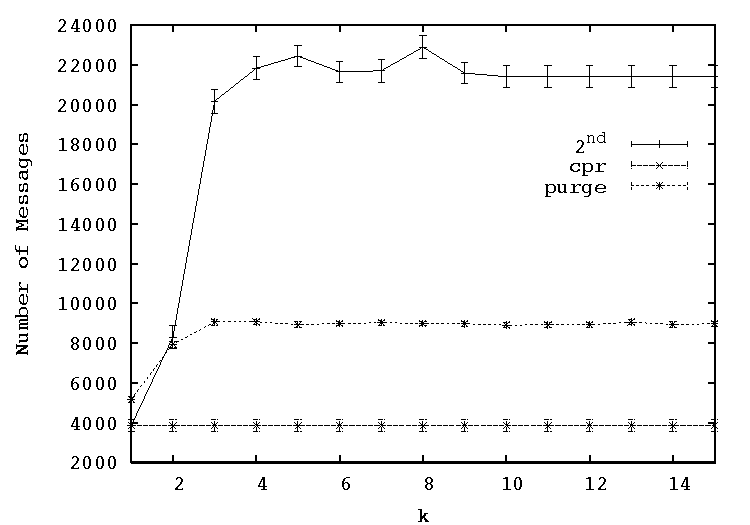
\includegraphics[width=0.32\textwidth]{figs/synch/msg-rand15.pdf}}
\subfigure[{$p=0.25$, diameter=$2.99$}]{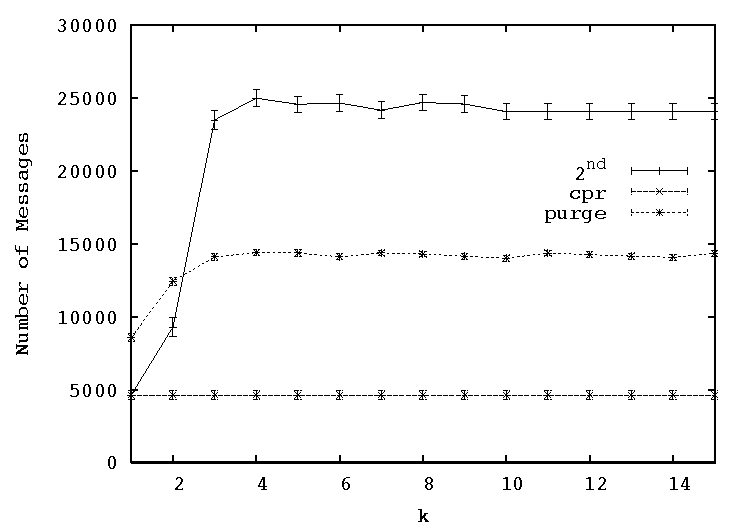
\includegraphics[width=0.32\textwidth]{figs/synch/msg-rand25.pdf}}
\subfigure[{$p=0.50$, diameter=$2$}]{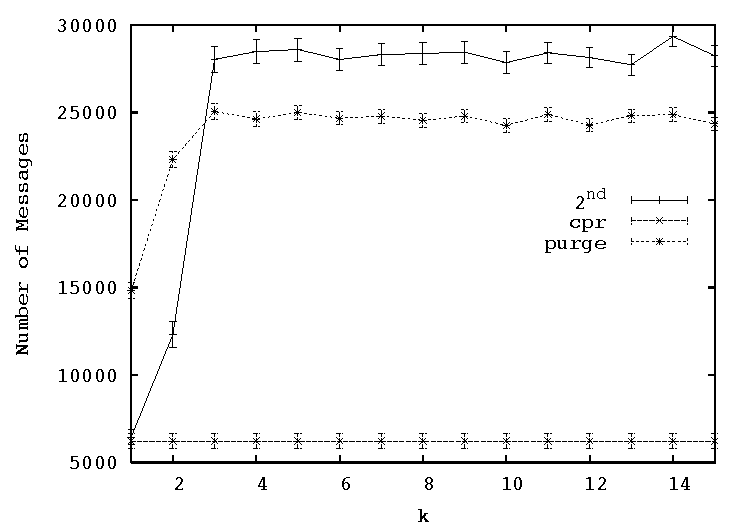
\includegraphics[width=0.32\textwidth]{figs/synch/msg-rand50.pdf}}
\caption{Experiment 2: message overhead for \er graph with link weights selected uniformly random from $[1,100]$. Note the y-axis have different scales.}
\label{fig:msg-rand}
\end{figure*}

%\begin{figure*}[t]
%\centering
%\subfigure[{$p=0.05$, diameter=$6.14$}]{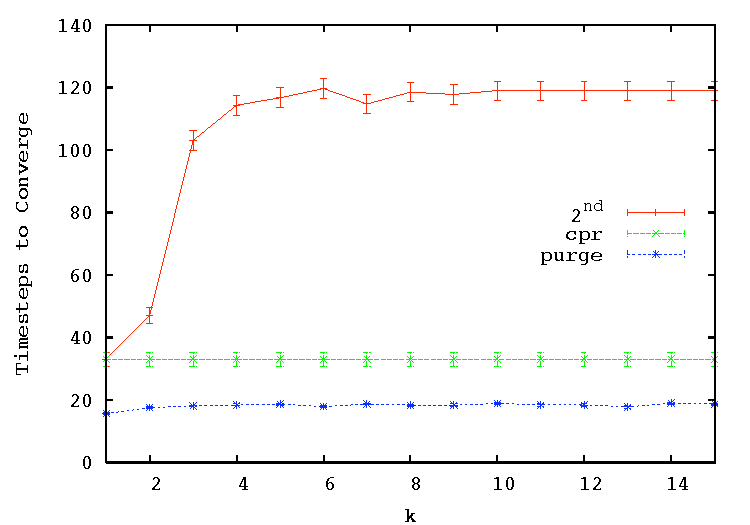
\includegraphics[width=0.32\textwidth]{figs/synch/epoch-rand5.pdf}}
%\subfigure[{$p=0.15$, diameter=$3.01$}]{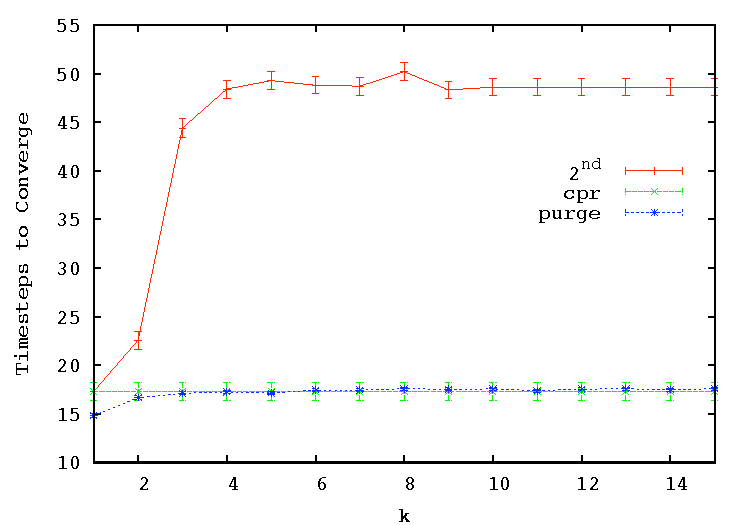
\includegraphics[width=0.32\textwidth]{figs/synch/epoch-rand15.pdf}}
%\subfigure[{$p=0.25$, diameter=$2.99$}]{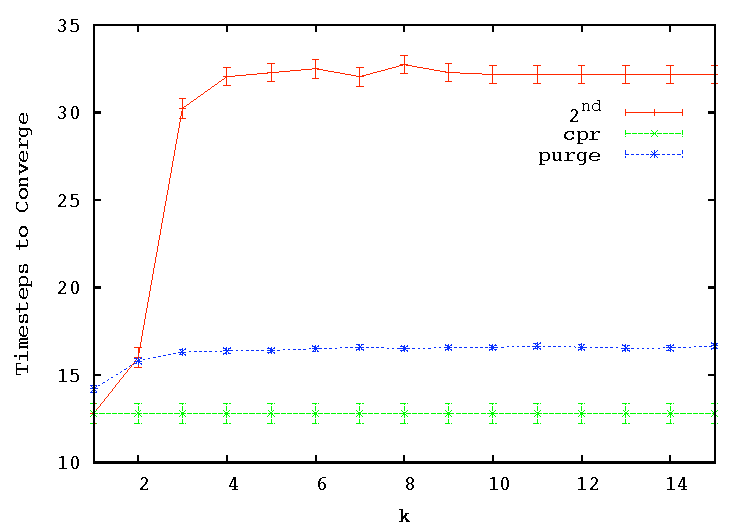
\includegraphics[width=0.32\textwidth]{figs/synch/epoch-rand25.pdf}}
%\subfigure[{$p=0.50$, diameter=$2$}]{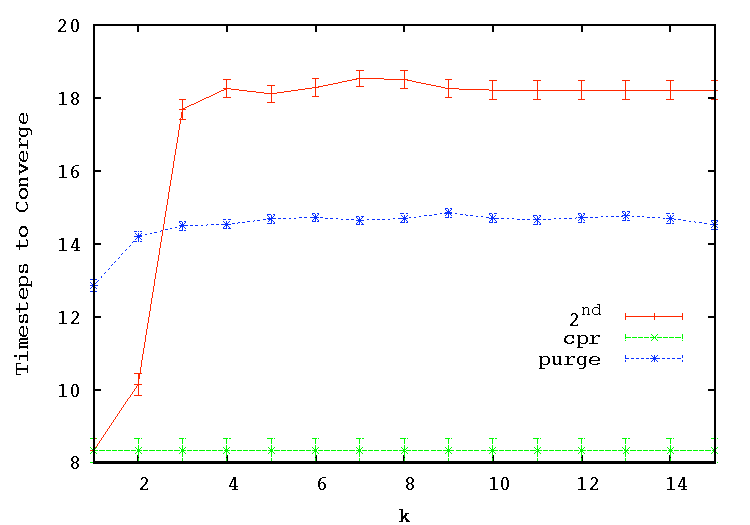
\includegraphics[width=0.32\textwidth]{figs/synch/epoch-rand50.pdf}}
%\subfigure[{Cumulative path cost decreases during the simulation}]{\includegraphics[width=0.49\textwidth]{figs/tsdecrease6.pdf}}
%\caption{Time overhead for \er graph with link weights selected uniformly random from $[1,100]$}
%\label{fig:epoch-rand}
%\end{figure*} 

%Recall that in Experiment 1, no pairwise routing loops are found when $p=0.15,p=0.25,$ and $p=0.50$.  The only pairwise routing loops in Experiment 1 
%are found when $p=0.05$, where a maximum of only $100$ pairwise routing loops occur. For \purges, no pairwise routing loops were found. {\bf Self-note}: {\it verify}.

In addition, we counted the number of epochs in which at least one pairwise routing loop existed.  For \second (across all topologies), on average, all but the last three 
timesteps had at least one routing loop.  This suggests that the \infinity problem dominates the cost for \seconds. 
%In some cases (e.g., $k=1$ for $p=.15$ and $p=.50$) \second performs better than \purges.  In these cases, \second has few routing loops.
%Table \ref{tab:loop} shows that there are fewer routing loops for small $k$. This is the case because with small $k$ there are fewer nodes using \badvectors. 

%The performance gap between \second and \purge shrinks with larger $p$ because with \second there are fewer routing loops with larger $p$.  
%This is consistent with our intuition:  larger $p$ values imply there are more alternate paths that do not use \badvectors.
%and thus routing loops are quickly exited because a low cost alternate path is used. 





\subsubsection{Experiment 3 - Internet-like Topologies}

%\begin{figure*}[t]
%\centering
%\subfigure[{AT\&T}]{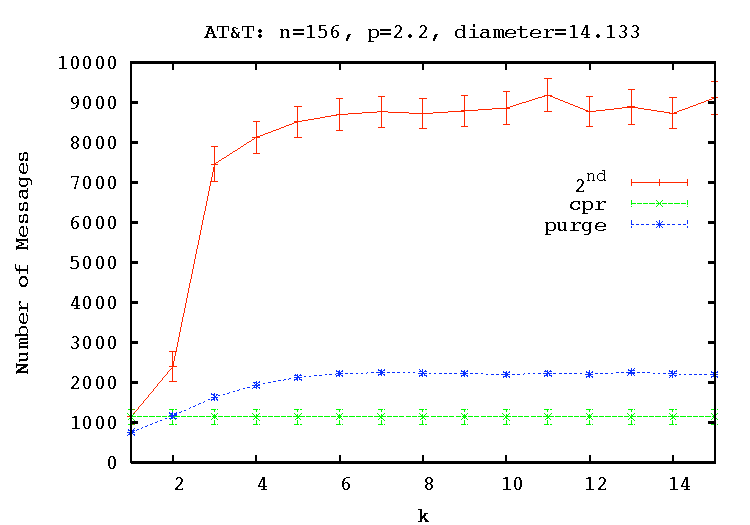
\includegraphics[width=0.32\textwidth]{figs/synch/att-msg.pdf}}
%\subfigure[{Rocketfuel 6461}]{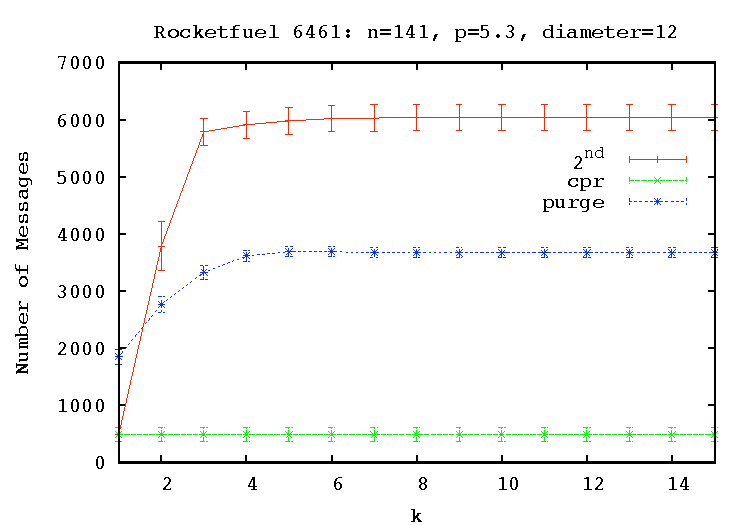
\includegraphics[width=0.32\textwidth]{figs/synch/rocket-msg6461.pdf}}
%\subfigure[{Rocketfuel 3867}]{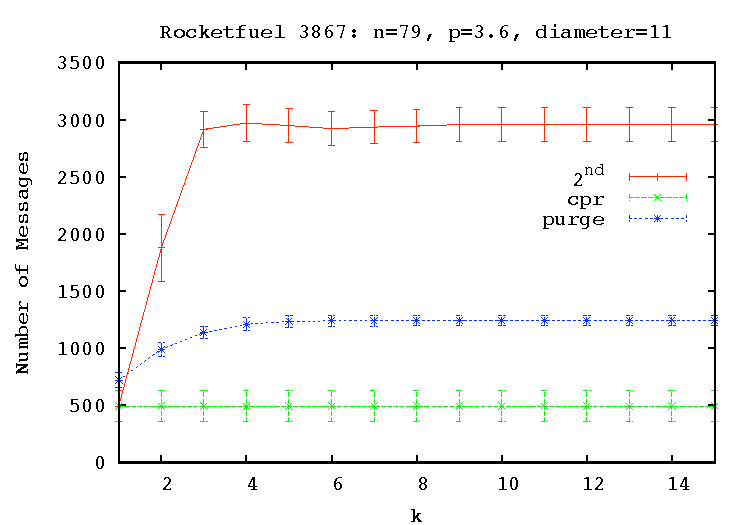
\includegraphics[width=0.32\textwidth]{figs/synch/rocket-msg3867.pdf}}
%\subfigure[{Cumulative path cost decreases during the simulation}]{\includegraphics[width=0.49\textwidth]{figs/tsdecrease6.pdf}}
%\caption{Real graph message overhead}
%\label{fig:msg-real}
%\end{figure*}


\begin{figure*}[t]
\centering
\subfigure[{GT-ITM, $n=156$, diameter=$14.133$}]{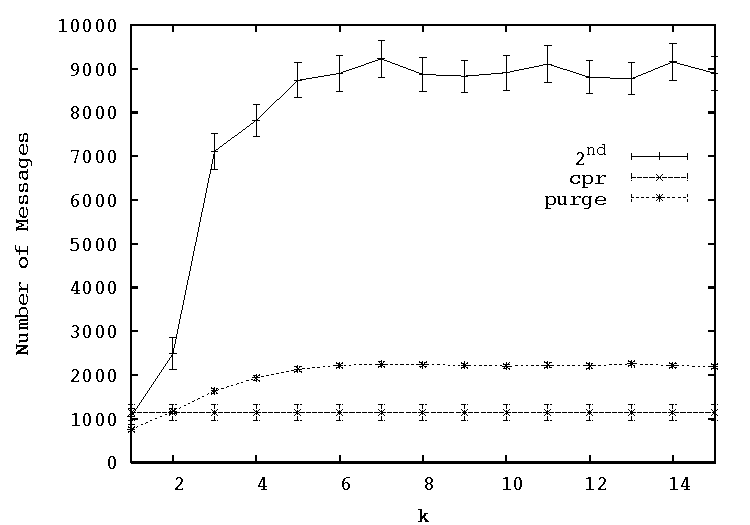
\includegraphics[width=0.32\textwidth]{figs/synch/msg-att.pdf}}
\subfigure[{Rocketfuel 6461, $n=141$, diameter=$8$}]{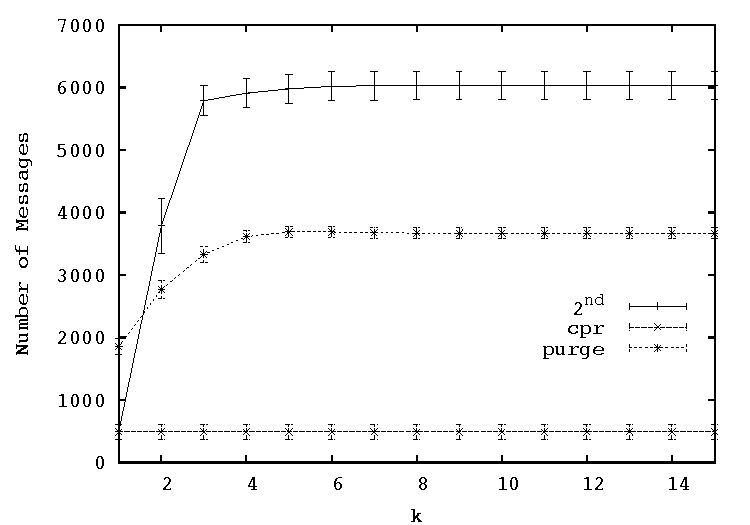
\includegraphics[width=0.32\textwidth]{figs/synch/msg6461.pdf}}
\subfigure[{Rocketfuel 3867, $n=79$, diameter=$10$}]{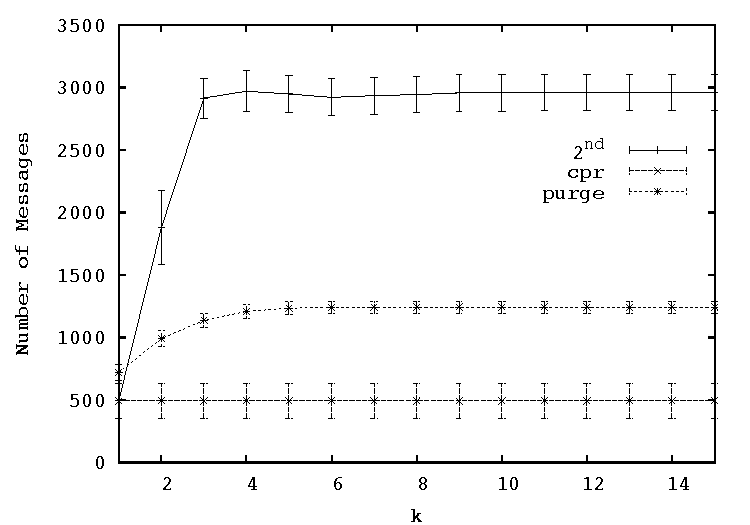
\includegraphics[width=0.32\textwidth]{figs/synch/msg3867.pdf}}
\caption{Experiment 3: Internet-like graph message overhead}
\label{fig:msg-real}
\end{figure*}

%\begin{figure*}[t]
%\centering
%\subfigure[{GT-ITM, $n=156$, average node degree=$2.2$, diameter=$14.133$}]{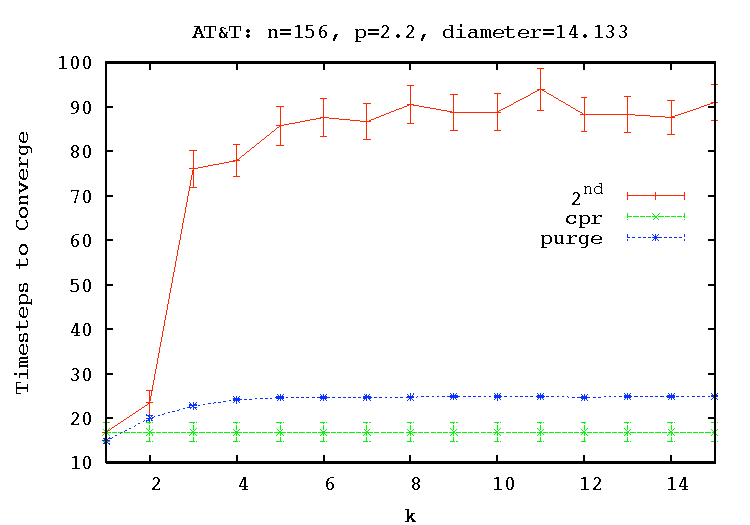
\includegraphics[width=0.32\textwidth]{figs/synch/att-epoch.pdf}}
%\subfigure[{Rocketfuel 6461, $n=141$, average node degree=$2.62$, diameter=$12$}]{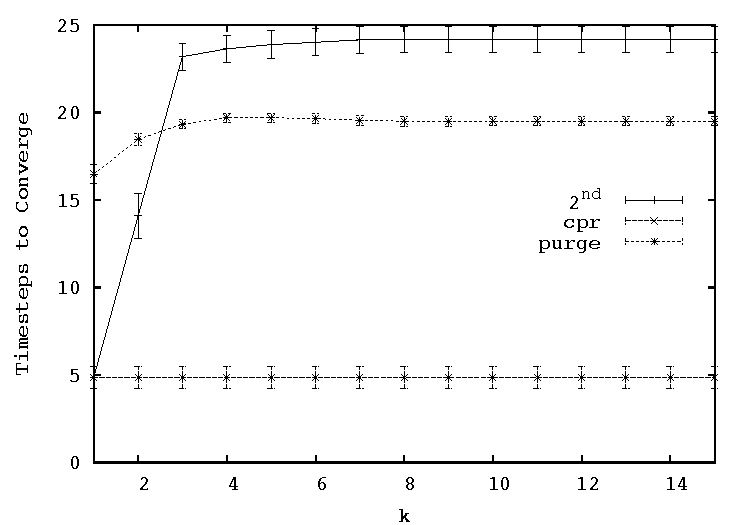
\includegraphics[width=0.32\textwidth]{figs/synch/rocket-epoch6461.pdf}}
%\subfigure[{Rocketfuel 3867, $n=79$, average node degree=$1.8$, diameter=$10$}]{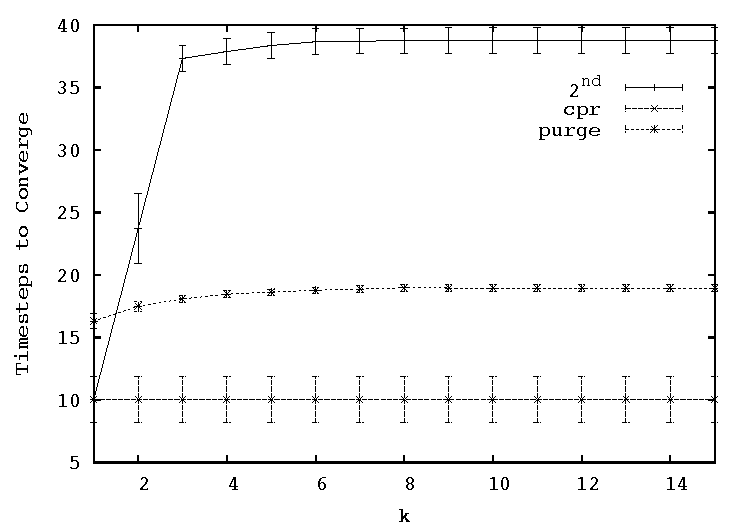
\includegraphics[width=0.32\textwidth]{figs/synch/rocket-epoch3867.pdf}}
%\subfigure[{Cumulative path cost decreases during the simulation}]{\includegraphics[width=0.49\textwidth]{figs/tsdecrease6.pdf}}
%\caption{Number of epochs/timesteps for real graphs}
%\label{fig:epoch-real}
%\end{figure*} 



Thus far, we studied the performance of our recovery algorithms over \er graphs, which have provided us with useful intuition about the performance
of each algorithm. In this experiment, we simulate our algorithms over Internet-like topologies downloaded from the Rocketfuel website \cite{Rocketfuel} and generated using GT-ITM 
\cite{GT-ITM}.  The Rocketfuel topologies have inferred edge weights. For each Rocketfuel topology, we let each node be
the compromised node and average over all of these cases for each value of $k$.  For GT-ITM, we used the parameters specified in Heckmann et al \cite{Heckmann} for  the $154$-node AT\&T topology
described in Section 4 of \cite{Heckmann}. For the GT-ITM topologies, we use the same criteria specified in Experiment 1 to generate each data point. 

The results, shown in Figure \ref{fig:msg-real}, follow the same pattern as in Experiment 2.  
%Due to space limitations, we only show the results for one representative topology.  The results for the other topologies follow the same pattern \cite{Tech}. 
In the cases where \second performs poorly,
the \infinity problem dominates the cost, as evidenced by the number of pairwise routing loops. In the few cases that \second performs better than \purges, there 
are few pairwise routing loops.

\subsubsection{Experiment 4 - Multiple Compromised Nodes}
\label{subsubsec:many}

In this experiment, we evaluate our recovery algorithms when multiple nodes are compromised. Our experimental setup is different from what we have used to this point:
we fix $k=\infty$ and vary the number of compromised nodes. Specifically, for each topology we create $m = \{1,2, ... , 15\}$ compromised nodes, each of which is selected  
uniformly at random (without replacement).  We then simulate the scenario described at the start of Section \ref{sec:eval} with one modification: $m$ nodes are 
compromised during $[t',t'+ 10]$. %We set $\Delta$ such that the recovery algorithm does not need to be restarted (as described in Section \ref{subsec:mult}).
The simulation is setup so that the outside algorithm identifies all $m$ compromised node at time $t$. %This eliminates the need to terminate and restart any recovery algorithm.
After running the simulation for all possible values for $m$, we generate a new topology and repeat the above procedure. 
We continue sampling topologies until the $90\%$ confidence interval for message overhead falls within $10\%$ of the mean message overhead. 

First, we perform this experiment using \er graphs with fixed link costs.  The message overhead results are shown in Figure \ref{fig:many-fixed}(a) for $p=0.05$ and $n=100$. 
{\footnote {\small We do not include the results for $p=\{0.15,0.25,0.50\}$ because they are consistent with the results for $p=0.05$.}}
The relative performance of the three algorithms is consistent with the results from Experiment 1, in which we had a single compromised node.
%We find the same trends we observed in Experiment 1 for large $k$ values in which there was a single compromised node.
As in Experiment 1, \second and \cpr have few pairwise routing loops (Figure \ref{fig:many-fixed}(b)).  In fact, there is more than an order of magnitude fewer pairwise routing 
loops in this experiment
when compared to the results for the same simulation scenario of $m$ compromised nodes using \er graphs with random link weights (Figure \ref{fig:many}(b)).
%The small number of pairwise routing loops is particularily evident when contrasted with the large number of pairwise routing loops 
%found with \er graphs with random link weights (Figure \ref{fig:many}(b)).  
Few routing loops imply that \second and \cpr (after rolling back) quickly count up to correct least costs.
In contrast, \purge has high message overhead because \purge globally invalidates false state before computing new least cost paths, rather than directly using alternate paths that 
are immediately available when recovery begins at time $t$. 
%The diffusing compuations are unnecessary in this scenario because many new least cost paths can be computed using local state information (demonstrated by \seconds's performance).

\second and \purge message overhead are nearly constant for $m \geq 8$ because at that point \badvector state has saturated $G$.
Figure \ref{fig:many-fixed} shows the number of least cost paths, per node,
that use \badvector or \oldvector at time $t$ (e.g., after \badvector state has propagated $k$ hops from \bads).  The number of least cost paths that use \badvector is nearly constant for $m \geq 8$. 

In contrast, \cpr message overhead increases with the number of compromised nodes.  After rolling back, \cpr must remove all compromised nodes and all
stale state (e.g., \oldvectors) associated with each \bads. As seen in Figure \ref{fig:many-fixed}(c), 
the amount of \oldvector state increases as the number of compromised nodes increase. 

Next, we perform the same experiment using \er graphs with with link weights selected uniformly at random from $[1,100]$. We only show the results for $p=.05$ and $n=100$ because the 
trends are consistent for other values of $p$.
The message overhead results for this experiment are shown in Figure \ref{fig:many}(a). \purge performs best because, unlike \second and \cprs, \purge does not suffer 
from the \infinity problem.  Below, we explain the performance of each algorithm in detail.

Consistent with Experiment 2 and 3, \second performs poorly because of the \infinity problem. 
Figure \ref{fig:many}(b) shows that a significant number of pairwise routing loops occur during \second recovery.  
\second message overhead remains constant when $m \geq 6$ because at this point \badvector state has saturated the network.  
Figure \ref{fig:many}(c) confirms this: the number of effected least cost paths remains constant (at $80$) for 
all $m \geq 6$. 

%\cpr also has a significant number of pairwise routing because after rolling back \cpr uses
%standard distance vector to compute new least cost paths for all paths using stale \oldvector state. Figure \ref{fig:many}(b) shows that the amount of \oldvector state increases as the
%number of compromised nodes increase, resulting in more routing loops for \cprs.

\cpr message overhead increases with the number of compromised nodes because the amount of \oldvector state increases as the number of compromised nodes increase (Figure \ref{fig:many}(c)). 
More \oldvector state results in more routing loops -- as shown in Figure \ref{fig:many}(b) -- causing increased message overhead.

%As with previous experiments,
\purge performs well because unlike \cpr and \seconds, no routing loops occur during recovery. %Figure \ref{fig:many}(b) shows that many pairwise routing loops occur during \second and \cpr recovery. 
Surprisingly, \purges's message overhead decreases when $m \geq 5$.  Although more 
least cost paths need to be computed with larger $m$, the message overhead decreases because the residual graph, $G'$, -- resulting from the removal of all $m$ compromised nodes -- is 
smaller than $G$.  As a result, there are $m$ fewer destinations and $m$ fewer nodes sending messages during the recovery process.
%As seen in Figure \ref{fig:many}(b), pairwise routing loops are prominent with both \second and \cprs. 

%used same topology for Rocketfuel ...
Finally, we simulated the same scenario of $m$ compromised node using the Internet-like graphs from Experiment 3. 
%{\footnote {\small For each Rocketfuel topology, we repeatidly selected $m$ compromised nodes until }}
The results were consistent with those for \er graphs with random link weights. % and therefore we do not present results for Internet-like graphs with multiple compromised nodes.



%Figure \ref{fig:many}(b) shows that the number of pairwise routing loops increases as the number of compromised nodes increases.  When $m \geq 6$, 
%in additional message overhead because more routing loops are processed per message. 
%{\bf think i want to remove the section about infinity message plot and the explanation about the number of loops per message}

\begin{figure*}[t]
\centering
\subfigure[{Message Overhead}]{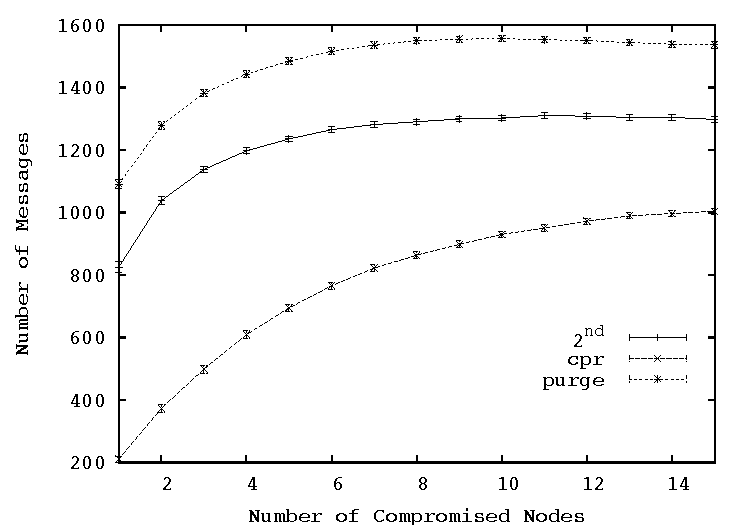
\includegraphics[width=0.32\textwidth]{figs/synch/many-fixed.pdf}}
\subfigure[{Pairwise Routing Loops}]{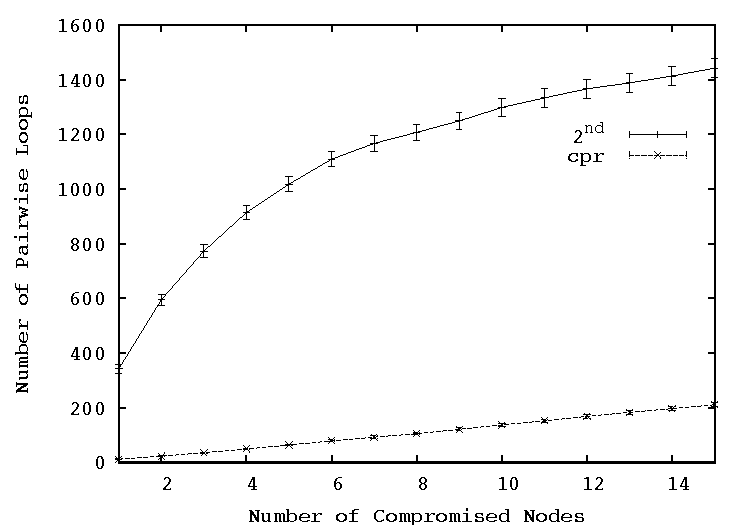
\includegraphics[width=0.32\textwidth]{figs/synch/loops-fixed.pdf}}
\subfigure[{Number of Effected Least Cost Paths}]{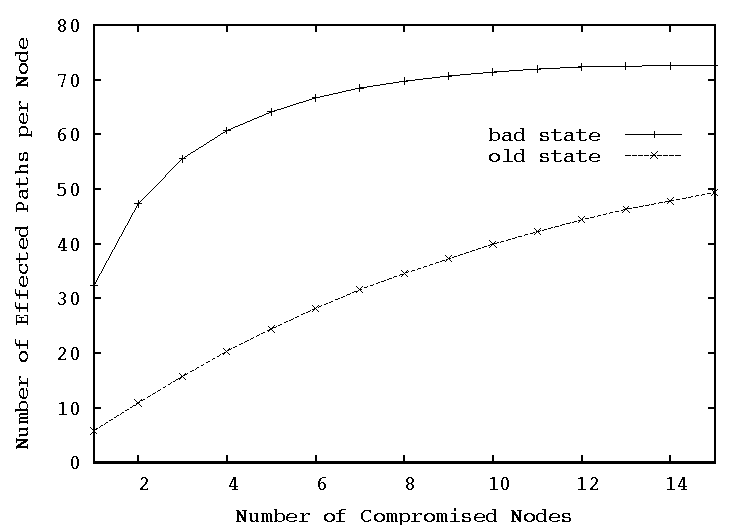
\includegraphics[width=0.32\textwidth]{figs/synch/initial-fixed.pdf}}
\caption{Experiment 4 - multiple compromised nodes over \er graphs with fixed link weights, $p=.05$, $n=100$, and diameter=$6.14$.}
\label{fig:many-fixed}
\end{figure*}



\begin{figure*}[t]
\centering
\subfigure[{Message Overhead}]{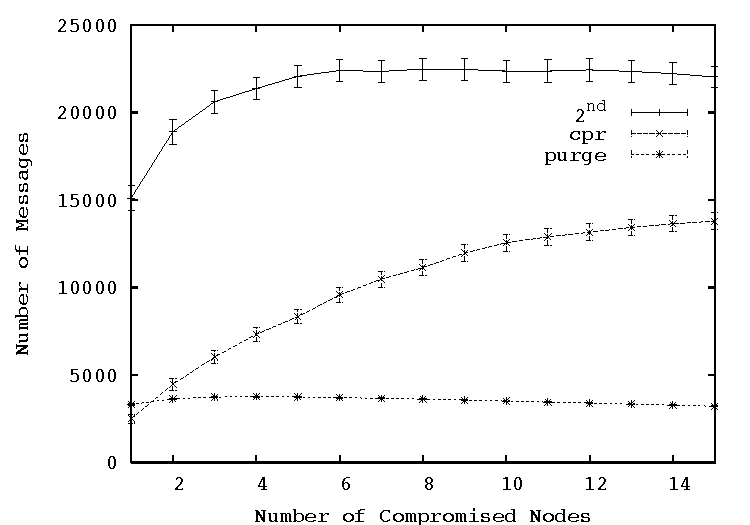
\includegraphics[width=0.32\textwidth]{figs/synch/many-rand.pdf}}
\subfigure[{Pairwise Routing Loops}]{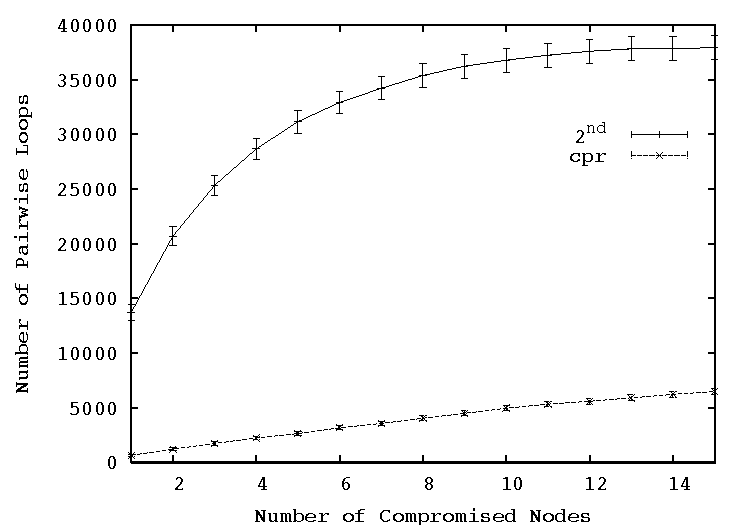
\includegraphics[width=0.32\textwidth]{figs/synch/loops-rand.pdf}}
\subfigure[{Number of Effected Least Cost Paths}]{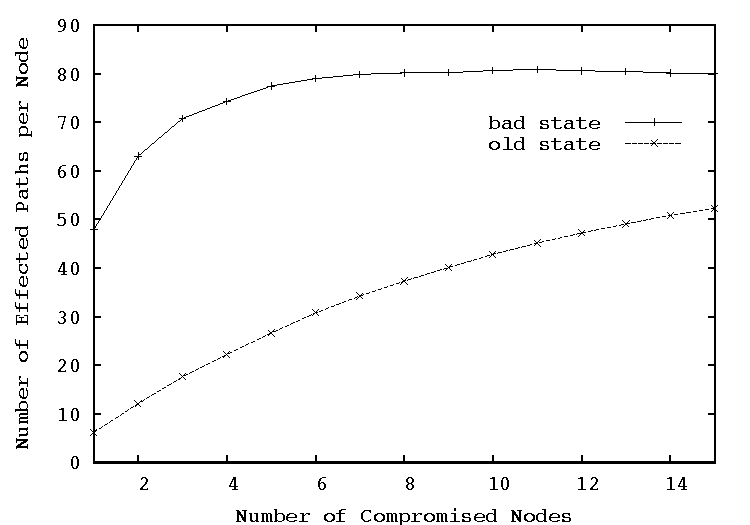
\includegraphics[width=0.32\textwidth]{figs/synch/initial-rand.pdf}}
\caption{Experiment 4 - multiple compromised nodes over \er graphs with link weights selected uniformly at random from $[1,100]$, $p=.05$, $n=100$, and diameter=$6.14$.}
\label{fig:many}
\end{figure*}

\subsubsection{Experiment 5 - Poison Reverse}
%Here we study the benefits of using poison reverse to \second and \cprs. 
We repeat Experiments 2, 3, and 4 using poison reverse for \second and \cprs.  
We do not apply poison reverse to \purge because no routing loops (resulting from the removal of \bads)
exist during \purges's recovery. Additionally, we do not repeat Experiment 1 using poison reverse because we observed few routing loops in that experiment. 

First, we repeat Experiment 2 using poison reverse. The results are shown for one representative topology in Figure \ref{fig:pr-fix}(a),
where \second + {\tt pr} and \cpr + {\tt pr} refer to each respective algorithm
using poison reverse. % The results are consistent for the other topologies considered in Experiments 2 and 3. %\er graphs with other $p$ values and for Internet-like topologies. 

\cpr + {\tt pr} has modest gains over standard \cpr because few routing loops occur with \cprs. On other hand,
\second + {\tt pr} sees a significant decrease in message overhead when compared to the standard \second algorithm because poison reverse removes the many pairwise routing 
loops that occur during \second recovery. However,  \second + {\tt pr} still performs worse than \cpr + {\tt pr} and \purges.  When compared to \cpr + {\tt pr}, 
the same reasons described in Experiment 2 account for \second + {\tt pr}'s poor performance. %high message complexity.  %reverse does not remove routing loops larger than $2$. 
Comparing \purge and \second + {\tt pr} yields interesting insights into the two different approaches for eliminating routing loops: \purge prevents routing loops using diffusing computations
and \second + {\tt pr} uses poison reverse.
Because \purge has lower message complexity than \second + {\tt pr} and poison reverse only eliminates pairwise routing loops, 
it suggests that \purge removes routing loops larger than $2$.
We are currently investigating this claim.

Repeating Experiment 3 using poison reverse yields the same trends as repeating Experiment 2 with poison reverse.  Finally, we consider poison reverse in the case 
of multiple compromised nodes (e.g., we repeat Experiment 4). \second + {\tt pr} and \cpr + {\tt pr} over \er graphs with unit link weights perform only slightly 
better than the basic version of each algorithm, respectively.  This is expected because few pairwise routing loops occur in this scenario.  

Like the single compromised node scenario, in the case of multiple compromised nodes, \second + {\tt pr} and \cpr + {\tt pr} over \er graphs with random link weights provide 
significant improvements over the basic version of each algorithm.  Particularly for \seconds, we observed many pairwise loops in Experiment 4 (Figure \ref{fig:many}(b)). This 
accounts for the effectiveness of poison reverse in this experiment.  Despite the significant improvements, \second + {\tt pr} still performs worse than \cpr + {\tt pr} and \purges. 
\cpr + {\tt pr} performs best among all the recovery algorithms because, as we have discussed, rolling back to a network-wide checkpoint is more efficient than using distance vector's
iterative procedure. Furthermore, poison reverse helps \cpr + {\tt pr} reduce the \infinity problem, improving \cprs's effectiveness in the face of multiple 
compromised nodes. 


\begin{figure*}[t]
\centering
%\subfigure[{Experiment 1}]{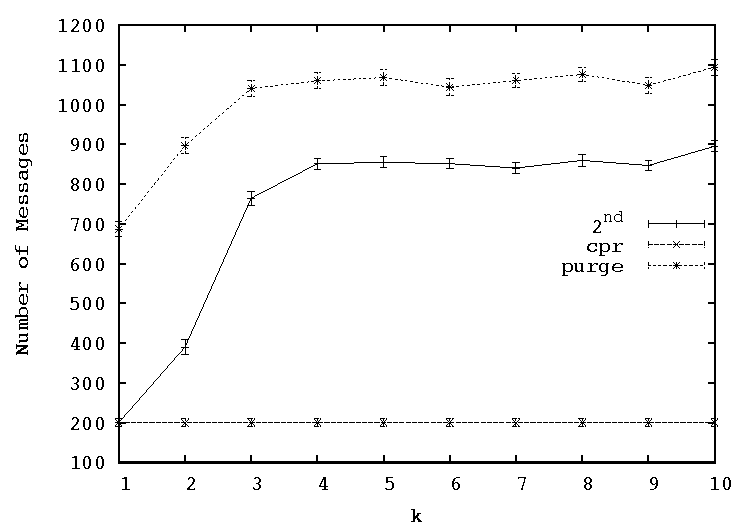
\includegraphics[scale=0.47]{figs/synch/msg5.pdf}}
%\subfigure[{Experiment 2 and 4}]{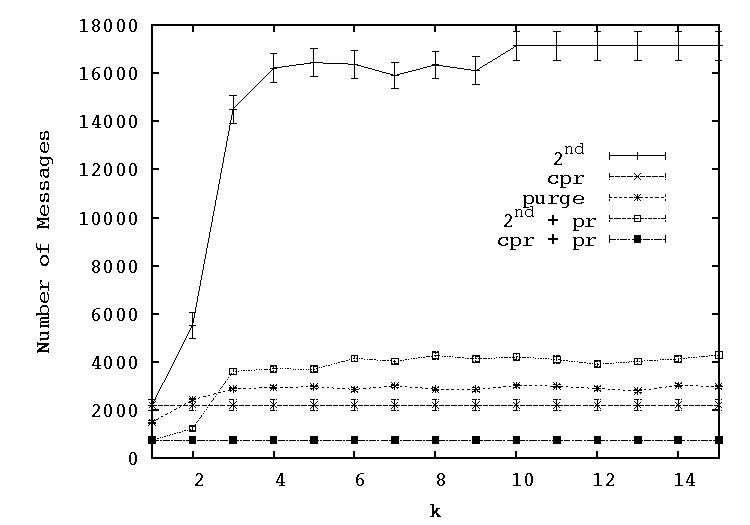
\includegraphics[scale=0.48]{figs/synch/msg-rand-pr5.pdf}}
%\subfigure[{Experiment 1}]{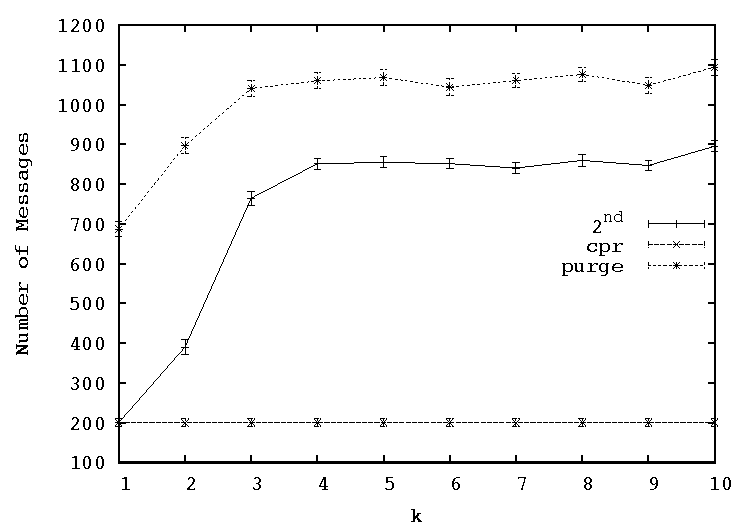
\includegraphics[width=0.49\textwidth]{figs/synch/msg5.pdf}}
\subfigure[{Single Compromised Node}]{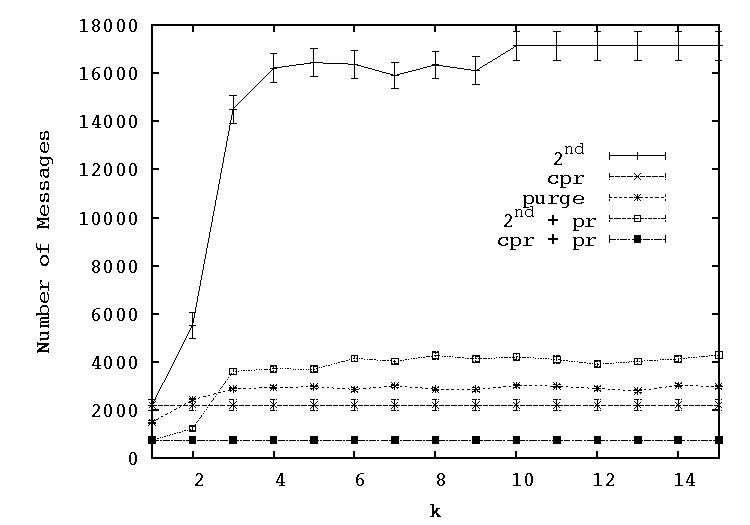
\includegraphics[width=0.32\textwidth]{figs/synch/msg-rand-pr5.pdf}}
\subfigure[{Multiple Compromised nodes}]{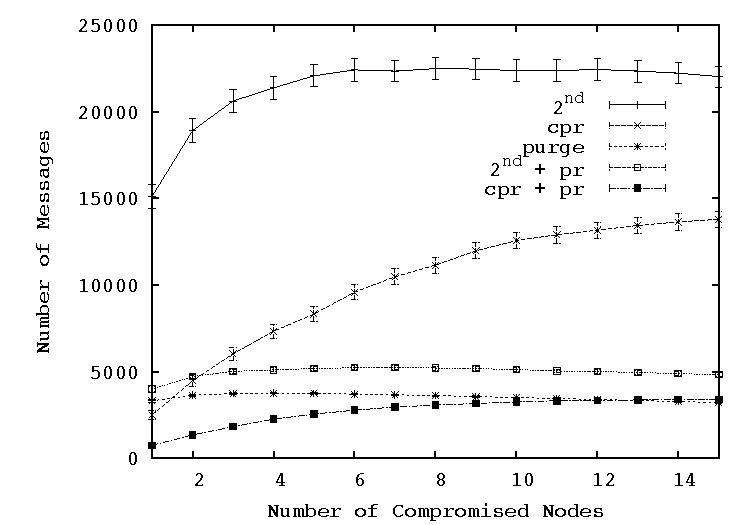
\includegraphics[width=0.32\textwidth]{figs/synch/many-pr-rand5.pdf}}
\caption{Experiment 5 plots.  Algorithms run over \er graphs with random link weights, $n=100$, $p=.05$, and average diameter=$6.14$. 
\second + {\tt pr} refers to \second using poison reverse. Likewise, \cpr + {\tt pr} is \cpr using poison reverse.}
\label{fig:pr-fix}
\end{figure*}




\subsection{Link Weight Change Experiments}
\label{subsec:change}

So far, we have evaluated our algorithms over different topologies with fixed link costs in scenarios with single and multiple compromised nodes.
We found that \cpr using poison reverse outperforms the other algorithms because \cpr removes false
routing state with a single diffusing computation, rather than using an iterative distance vector process as in \second and \purges, and poison reverse removes
all pairwise routing loops that occur during \cpr recovery. 

In the next three experiments we evaluate our algorithms over graphs with changing link costs. We introduce link cost changes between the time \bad is compromised and when \bad is discovered 
(e.g., during $[t',t_b]$). 
In particular, let there be $\lambda$ link cost changes per timestep, where $\lambda$ is deterministic. 
To create a link cost change event, we choose a link (except for all $(v,\bar{v})$ links) whose link will change equiprobably among all links. 
The new link cost is selected uniformly at random from $[1,n]$. 

\subsubsection{Experiment 6 - Link Cost Changes}

Except for $\lambda$, our experimental setup is identical to the one in Experiment 2. We let $\lambda = \{1,4,8\}$. In order to isolate the effects of link costs changes,
we assume that \cpr checkpoints at each timestep.

Figure \ref{fig:lc} shows \purge yields the lowest message overhead for $p=.05$, but only slightly lower than \cprs. 
\cprs's message overhead increases with larger $k$ because there are more link cost change events to process. After \cpr rolls back, it must process all link cost
changes that occurred in $[t',t_b]$. 
In contrast, \second and \purge process some of the link cost change events during the interval $[t',t_b]$ as part of normal distance vector execution. 
In our experimental setup, these messages are not counted because 
they do not occur in Step 4 (i.e., as part of the recovery process) of our simulation scenario described in Section \ref{sec:eval}.

Our analysis further indicates that \second performance suffers because of the \infinity problem. %\purge and \second must 
The gap between \second and the other algorithms shrinks as $\lambda$ increases because as $\lambda$ increases, link cost changes have a larger effect on message overhead.


\begin{figure*}[t]
\centering
\subfigure[{$p=0.05$, diameter=$6.14, \lambda=1$}]{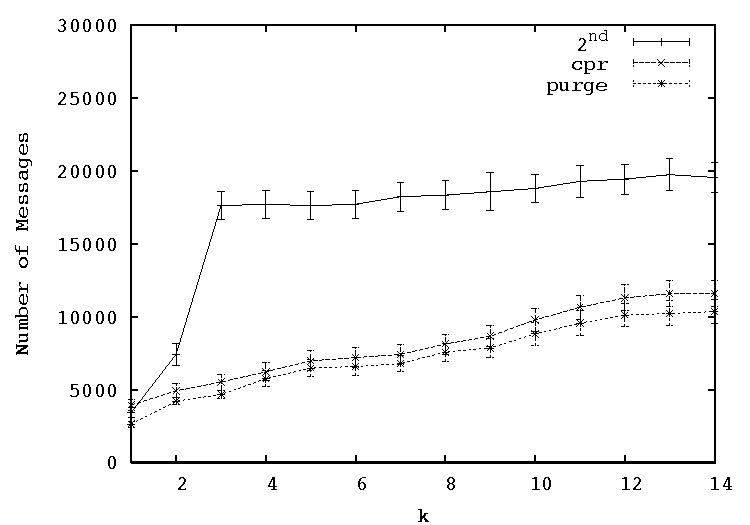
\includegraphics[width=0.32\textwidth]{figs/synch/p05-lc1.pdf}}
%\subfigure[{$p=0.05$, diameter=$6.14, \lambda=2$}]{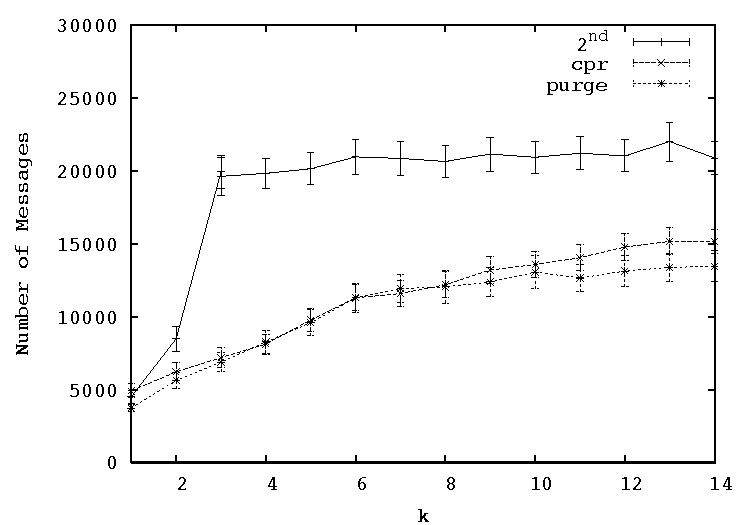
\includegraphics[width=0.32\textwidth]{figs/synch/p05-lc2.pdf}}
\subfigure[{$p=0.05$, diameter=$6.14,\lambda=4$}]{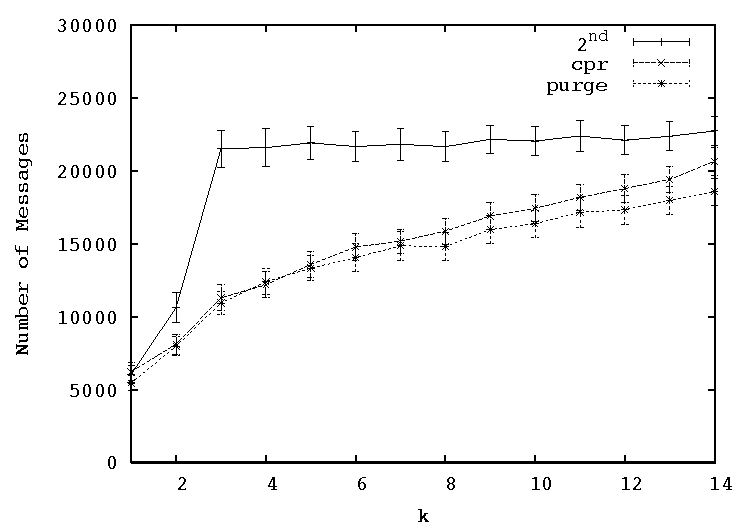
\includegraphics[width=0.32\textwidth]{figs/synch/p05-lc4.pdf}}
\subfigure[{$p=0.05$, diameter=$6.14, \lambda=8$}]{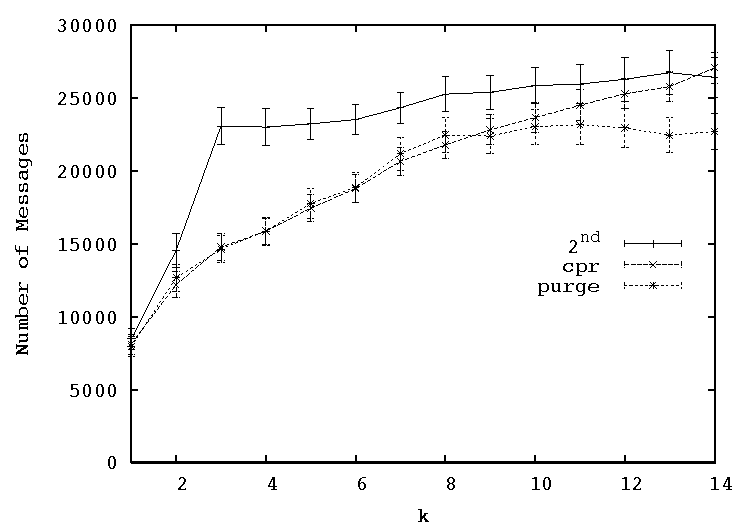
\includegraphics[width=0.32\textwidth]{figs/synch/p05-lc8.pdf}}
\subfigure[{$p=0.15$, diameter=$3.01, \lambda=1$}]{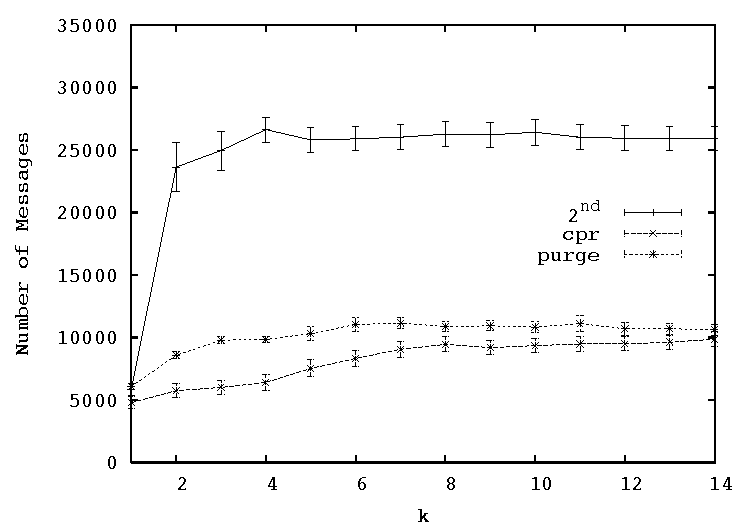
\includegraphics[width=0.32\textwidth]{figs/synch/p15-lc1.pdf}}
\subfigure[{$p=0.15$, diameter=$3.01,\lambda=4$}]{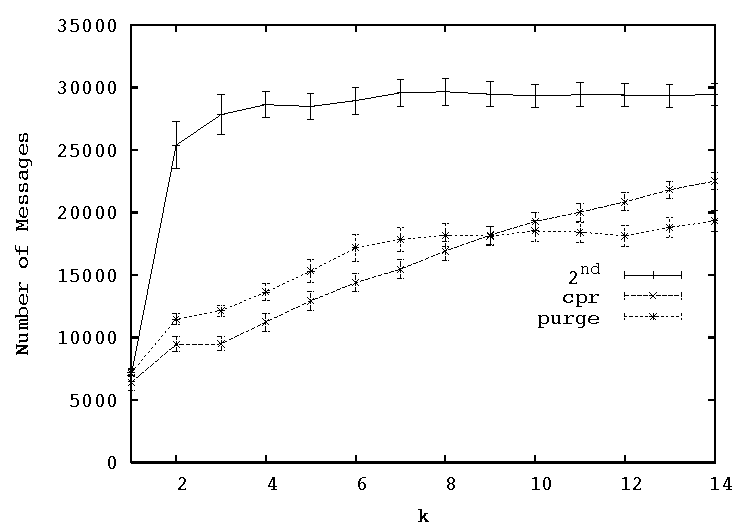
\includegraphics[width=0.32\textwidth]{figs/synch/p15-lc4.pdf}}
\subfigure[{$p=0.15$, diameter=$3.01, \lambda=8$}]{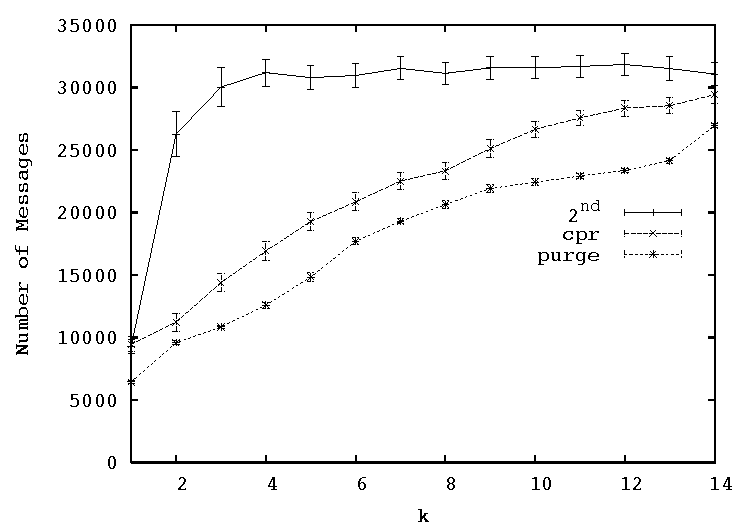
\includegraphics[width=0.32\textwidth]{figs/synch/p15-lc8.pdf}}
%\subfigure[{Cumulative path cost decreases during the simulation}]{\includegraphics[width=0.49\textwidth]{figs/tsdecrease6.pdf}}
\caption{Experiment 6: Message overhead for $p=\{0.05,0.15\}$ \er with link weights selected uniformly random with different $\lambda$ values.}
\label{fig:lc}
\end{figure*}

%\begin{figure*}[t]
%\centering
%\subfigure[{$p=0.15$, diameter=$3.01, \lambda=1$}]{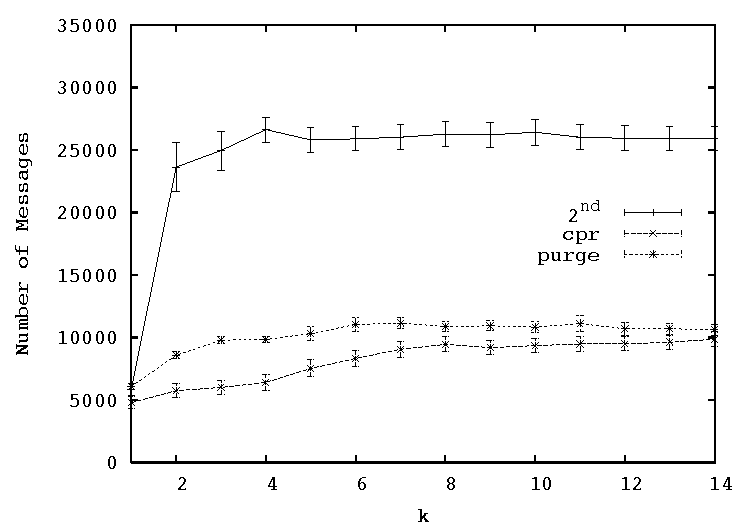
\includegraphics[width=0.32\textwidth]{figs/synch/p15-lc1.pdf}}
%\subfigure[{$p=0.15$, diameter=$3.01,\lambda=4$}]{\includegraphics[width=0.32\textwidth]{figs/synch/p15-lc4.pdf}}
%\subfigure[{$p=0.15$, diameter=$3.01, \lambda=8$}]{\includegraphics[width=0.32\textwidth]{figs/synch/p15-lc8.pdf}}
%\subfigure[{Cumulative path cost decreases during the simulation}]{\includegraphics[width=0.49\textwidth]{figs/tsdecrease6.pdf}}
%\caption{Message overhead for $p=0.15$ \er with link weights selected uniformly random with different $\lambda$ values.}
%\label{fig:lc-p15}
%\end{figure*} 

With larger $p$ values, $\lambda$ has a smaller effect on message complexity because more alternate paths are available. Thus when $p=0.15$ and $\lambda=1$,
most of \purges's recovery effort is towards removing \badvector state, rather than processing link cost changes.  Because
\cpr removes \badvector using a single diffusing computation and there are few link cost changes, \cpr has lower message overhead than \purge in this case. 
As $\lambda$ increases, \cpr has higher message overhead than \purges: there are more link cost changes to process and \cpr must process all such link cost changes, 
while \purge processes some link cost changes during the interval $[t',t_b]$ as part of normal distance vector execution. 

\subsubsection{Experiment 7 - Poison Reverse and Link Cost Changes}
In this experiment, we apply poison reverse to each algorithm and repeat Experiment 6. Because \purges's diffusing computations only eliminate routing loops corresponding 
to \badvector state, \purge is vulnerable to routing loops stemming from link cost changes.  Thus, contrary to Experiment 5, poison reverse improves \purge performance.
The results are shown in Figure \ref{fig:prlc}. Each algorithm using poison reverse has label ``{\tt algorithm-name}'' + {\tt pr}).
Results for different $p$ values yield the same trends. 

All three algorithms using poison reverse show remarkable performance gains.
As confirmed by our profiling numbers, the improvements are significant because routing loops are more pervasive when link costs change.  
Accordingly, the poison reverse optimization yields greater benefits as $\lambda$ increases. % because larger $\lambda$ result in more routing loops. %for the standard \second and \cpr algorithms.

%Each algorithm using poison reverse is vulnerable to routing loops larger than $2$ that originate from link cost changes,
As in Experiment 5, we believe that for \badvector state \emph{only}, \purge + {\tt pr} removes routing loops larger than $2$ while \second + {\tt pr} does not. 
For this reason, we believe that \purge + {\tt pr} performs better than \second + {\tt pr}.  We are currently investigating this claim.
%As in Experiment 3, \second + {\tt pr} performs worse than \purge + {\tt pr} because we believe that for \badvector state \emph{only},
%\purge + {\tt pr} removes routing loops larger than $2$ while \second + {\tt pr} does not. Meanwhile, both 
% \second + {\tt pr} and \purge + {\tt pr} use poison reverse to address routing loops resulting from link cost changes.  Thus both algorithms (and \cpr + {\tt pr})
%are equally vulnerable to routing loops  larger than $2$ originating from link cost changes.
\cpr + {\tt pr} has the lowest message complexity. %among the three algorithms. 
In this experiment, the benefits of rolling back to a global snapshot taken before \bad was compromised outweigh the message overhead required to update stale state pertaining to 
link cost changes that occurred during $[t',t_b]$. As $\lambda$ increases,
the performance gap decreases because \cpr + {\tt pr} must process all link cost changes that occurred in $[t',t_b]$ while \second + {\tt pr}  and \purge + {\tt pr}
process some link cost change events during $[t',t_b]$ as part of normal distance vector execution.

%However, we make the strong performance of \cpr + {\tt pr} comes wiHh
However, \cpr + {\tt pr} only achieves such strong results by making two optimistic assumptions:  we assume perfectly synchronized clocks and checkpointing occurs at each timestep.
In the next experiment we relax the checkpointing assumption.
%However, we make two optimistic assumptions in order to achieve such favorable results for \cpr + {\tt pr}: we assume clocks are perfectly synchronized and checkpointing occurs at each timestep.
%In the next experiment we relax the checkpoint assumption.


\begin{figure*}[t]
\centering
\subfigure[{$p=0.05$, $\lambda=1$}]{\includegraphics[width=0.32\textwidth]{figs/synch/pr-p05-lc1.pdf}}
%\subfigure[{$p=0.05, \lambda=2$}]{\includegraphics[width=0.49\textwidth]{figs/synch/p05-lc2.pdf}}
\subfigure[{$p=0.05$, $\lambda=4$}]{\includegraphics[width=0.32\textwidth]{figs/synch/pr-p05-lc4.pdf}}
\subfigure[{$p=0.05$, $\lambda=8$}]{\includegraphics[width=0.32\textwidth]{figs/synch/pr-p05-lc8.pdf}}
%\subfigure[{Cumulative path cost decreases during the simulation}]{\includegraphics[width=0.49\textwidth]{figs/tsdecrease6.pdf}}
\caption{Plots for Experiment 7. Each figure shows message overhead for \er graphs with link weights selected uniformly at random, $p=0.05$, average diameter is $6.14$, and $\lambda=\{1,4,8\}$.
The curves for \second + {\tt pr}, \purge + {\tt pr}, and \cpr + {\tt pr} refer to each algorithm using poison reverse, respectively.
} 
\label{fig:prlc}
\end{figure*}


\subsubsection{Experiment 8 - Vary Checkpoint Frequency}

In this experiment we study the trade-off between message overhead and storage overhead for \cprs. To this end, we vary the frequency at which \cpr checkpoints and fix 
the interval $[t',t_b]$. Otherwise, our experimental setup is the same as Experiment 6.

Figure \ref{fig:lc-fixk} shows the results for an \er graph with link weights selected uniformly at random between $[1,n]$,
$n=100$, $p=.05$, $\lambda=\{1,4,8\}$ and $k=2$. We plot message overhead against the number of timesteps \cpr must rollback, $z$. \cprs's message overhead increases with larger $z$ 
because as $z$ increases there are more link cost change events to process. \second and \purge have constant message overhead because they operate independent of $z$.

We conclude that as the frequency of \cpr snapshots decreases, \cpr incurs higher message overhead.  Therefore, when choosing the frequency of checkpoints,
the trade-off between storage and message overhead must be carefully considered. 



\begin{figure*}[t]
\centering
\subfigure[{$p=0.05$, $k=2, \lambda=1$}]{\includegraphics[width=0.32\textwidth]{figs/synch/p05-k1.pdf}}
\subfigure[{$p=0.05$, $k=2, \lambda=4$}]{\includegraphics[width=0.32\textwidth]{figs/synch/p05-k4.pdf}}
\subfigure[{$p=0.05$, $k=2, \lambda=8$}]{\includegraphics[width=0.32\textwidth]{figs/synch/p05-k8.pdf}}
%\subfigure[{Cumulative path cost decreases during the simulation}]{\includegraphics[width=0.49\textwidth]{figs/tsdecrease6.pdf}}
\caption{Experiment 8: message overhead for $p=0.05$ \er with link weights selected uniformly random with different $\lambda$ values. $z$ refers to the number of timesteps \cpr must 
rollback. Note the y-axis have different scales.}
\label{fig:lc-fixk}
\end{figure*} 


\subsection{Summary}
\label{subsec:discuss}


Our results show \cpr using poison reverse yields the lowest message and time overhead in all scenarios. \cpr benefits from removing false state with a single
diffusing computation. Also, applying poison reverse significantly reduces \cpr message complexity by eliminating pairwise routing loops resulting from
link cost changes. However, \cpr has storage overhead, requires loosely synchronized clocks, and requires the time \bad was compromised.

\seconds's performance is determined by the \infinity problem. In the case of \er graphs with fixed unit link weights, the \infinity problem was minimal, 
helping \second perform better than \purges. % In all other scenarios, poison reverse significantly improves \second performance because routing loops are pervasive.
For all other topologies, poison reverse significantly improves \second performance because routing loops are pervasive.
Still, \second using poison reverse is not as efficient as \cpr and \purge using poison reverse.

In cases where link costs change, we found that \purge using poison reverse is only slightly worse than \cpr + {\tt pr}. % with poison reverse. 
Unlike \cprs, \purge makes use of computations that follow the injection of false state, that do not depend on false routing state.  
Because \purge does not make the assumptions that \cpr requires, \purge using poison reverse is a suitable alternative for topologies with link cost changes.
%In contrast to \cprs, \purge makes no assumptions 
%other than the identification of \bads, making \purge a suitable algorithm for topologies with link cost changes.

%\purge avoids the \infinity problem by first globally invalidating false state.  Therefore in cases where the \infinity problem is 
%significant, \purge outperforms \seconds.

%When considering graphs with changing link costs, \cprs's performance suffers because it must process all valid link cost changes that occurred since \bad was compromised.
%Meanwhile, \second and \purge make use of computations that followed the injection of false state, that do not depend on false routing state. However, \seconds's performance degrades 
%because of the \infinity problem.  \purge eliminates the \infinity problem and therefore yields the best performance over topologies with changing link costs.

Finally, we found that an additional challenge with \cpr is setting the parameter which determines checkpoint frequency.
Frequent checkpointing yields lower message and time overhead at the cost of more storage overhead. Ultimately, application-specific factors must be considered
when setting this parameter. 
